\documentclass[10pt,a4paper]{article}
\usepackage[utf8]{inputenc}
\usepackage[english]{babel}
\usepackage{graphicx}
\usepackage{lmodern}
\usepackage{kpfonts}
\usepackage[left=2cm,right=2cm,top=2cm,bottom=2cm]{geometry}
\usepackage{dsfont}
\usepackage[noend]{algpseudocode}
\usepackage{wrapfig}
\usepackage{algorithm}
\newtheorem{theorem}{Theorem}
\newtheorem{definition}{Definition}
\newtheorem{notation}{Notation}
\author{Megi Dervishi}
\title{Algorithms and Programation}

\begin{document}

\maketitle
\section*{Homework 2 (30/10/2019)}
\subsection*{Exercise 1}
\subsection*{Solution}
\textbf{(1)}
\begin{algorithm}
\caption{Greedy Algorithm for $\{1,5,10,25,50\}$}\label{ed}
\begin{algorithmic}[1]
\Function{Coin\_ Change ($n$)}{}
	\State $\textit{q}_{50} \gets \lfloor n\, / 50 \rfloor$
	\State $\,  r_{50} \gets n \mod 50$
	\State $\,  q_{25} \gets \lfloor r_{50}\, / 25 \rfloor $
	\State $\, r_{25} \gets r_{50} \mod 25 \
	 $
	\State $\, q_{10} \gets \lfloor r_{25}\,  / 10\rfloor$
	\State $\, r_{10} \gets r_{25} \mod 10$
	\State $\, q_{5} \gets \lfloor r_{10}\,  / 5 \rfloor$
	\State $\, r_{5} \gets r_{10} \mod 5$
	\State $\, q_{1} \gets \lfloor r_{5}\, / 1 \rfloor$\\\Return $(q_1, q_5, q_{10}, q_{25}, q_{50})$
\EndFunction
\end{algorithmic}
\end{algorithm}
\\
\textbf{Proof of Correctness}\\\\
Let the optimal solution and greedy's algorithm solution be $$\text{OPT} = (a,b,c,d,e) \Rightarrow n = a + b\cdot 5 + c\cdot 10 + d\cdot 25 + e \cdot 50$$  $$\text{ALG} =(q_1, q_5, q_{10}, q_{25}, q_{50}) \Rightarrow  n = q_1 +  q_5\cdot 5 + q_{10}\cdot 10 + q_{25}\cdot 25 + q_{50}\cdot 50$$
where each coefficient represent the number of specific coins.
Let us analyze the coefficients of the optimal solution. We must have the following restrictions in order to have an optimal solution.
\begin{itemize}
\item $\mathbf{a < 5}\quad$       If $a \geq 5$ then we could substitute at least 5 coins with 1 coin of value 5 i.e optimal choice
\item $\mathbf{b < 2}\quad$      If $b \geq 2$ then we could substitute at least 2 coins with 1 coin of value 10 i.e optimal choice
\item $\mathbf{c < 3}\quad \,$        If $c \geq 3$ then we could substitute at least 3 coins with 1 coin of value 25 and 1 coin of 5 value
\item $\mathbf{d < 2}\quad$       If $d \geq 2$ then we could substitute at least 2 coins with 1 coin of value 50 i.e optimal choice
\item $\mathbf{e \in \mathbb{N}}\quad$
\item Finally we also have that $c + b < 3$ since if we have two coins of 10 and one coin of 5 we can replace it by one coin of 25.
\end{itemize}
Having these restriction we plug in the optimal $n$ in the algorithm.
\begin{itemize}
\item $$ q_{50} = \frac{n}{50} = \left\lfloor\frac{a + b\cdot 5 + c\cdot 10 + d\cdot 25 + e \cdot 50}{50}\right\rfloor = \Bigg\lfloor e + \underbrace{\frac{a}{50} + \frac{b}{10} + \frac{c}{5} + \frac{d}{2}}_{\leq \frac{4}{50} + \frac{1}{10} + \frac{1}{5} + \frac{1}{2} = 0.88 < 1}\Bigg\rfloor = e
$$
\item 
$$r_{50} = a + b\cdot 5 + c\cdot 10 + d\cdot 25 $$
$$q_{25} = \left\lfloor \frac{r_{50}}{25}\right\rfloor = d +\Bigg \lfloor \underbrace{\frac{a + b \cdot 5 + 10 \cdot c}{25}}_{\leq \frac{4 + 1 \cdot 5 + 1 \cdot 10}{25} = 0.76 < 1} \Bigg\rfloor = d$$
\item 
$$r_{25} = a + b\cdot 5 + c\cdot 10 $$
$$q_{10} = \left\lfloor\frac{r_{25}}{10}\right\rfloor = c + \Bigg\lfloor \underbrace{\frac{a + b\cdot 5}{10}}_{\leq \frac{4 + 1 \cdot 5}{10} = 0.9 < 1}  \Bigg\rfloor = c$$
\item 
$$r_{10} = a + b\cdot 5$$
$$q_{5} = \left\lfloor\frac{r_{10}}{5}\right\rfloor = b + \left\lfloor \frac{a}{5} \right\rfloor = b$$
\item $$r_{5} = a$$
$$q_{1} = \left\lfloor \frac{r_{5}}{1} \right\rfloor = a$$
\end{itemize}
Therefore with this particular set of denominations the solution of the greedy algorithm is the same as the optimal solution.
\subsubsection*{Time Complexity}
We observe that the algorithm is composed of 9 arithmetic operations which are done in constant time. Therefore this greedy algorithm takes $\mathcal{O}(1)$ times.\\\\
\textbf{(2)}\\\\
Using the above algorithm with the denominators $\{1,6,10\}$ and $n = 12$ we will obtain $(2, 0, 1)$ i.e. $3$ coins whereas the optimal solution would be $(0,2,0)$  i.e. 2 coins.\\\\
\textbf{(3)}\\\\
Let $D = \{d_1,d_2,\cdots d_k\}$. For the optimized algorithm we use dynamic programming i.e. a table $tab$ in which we will store the number of coins used for each subproblem and $bestcoin$ is an array that will store the particular $d_k$ used to give the optimal solution for each subproblem.\\
\textbf{Note}: The below pseudocode has the same indexes as a python program.\\\\
\textbf{Time complexity:}
The first loop of the algorithm is $\mathcal{O}(n)$ time and the second one is $\mathcal{O}(k)$ time; the last while loop is at most $\mathcal{O}(n)$ time. Therefore the total complexity is $\mathcal{O}(nk)$ time.
\begin{algorithm}
\caption{Optimized algorithm}\label{ed}
\begin{algorithmic}[1]
\Function{Coin\_ Change ($amount$, $D$)}{}
	\State $n \gets amount + 1$
	\State $tab \gets [n]*n$ 
   	\State $tab[0] \gets 0$
   	\State $bestcoins \gets [0]*n$
   	\For {$i \gets 1 \text{ to } n +1$}
        \State $c \gets 0$  
        \For {$k  \gets 0 \text{ to  length of } D$}
           \If {$tab[i] > tab[i-D[k]]+1$}
                \State $c \gets D[k]$
                \State $tab[i] \gets tab[i-D[k]]+1$
            \EndIf
        \State $bestcoins[i] \gets c$
        \EndFor
    \EndFor
    	\If {$tab[amount] > amount$} \Return "No change" \EndIf
    \State $result \gets [\,]$
    \State $i \gets amount$
    \While  {$i > 0$} {
        \State \textbf{append } $bestcoins[i]$ \textbf{ to } $result$
        \State $i \gets i - bestcoins[i]$
    \EndWhile}
    \Return $result$
\EndFunction
\end{algorithmic}
\end{algorithm}
\newpage

\subsection*{Exercise 2}
\subsection*{Solution}
\textbf{(1)}\\\\
The naive multiplication of the matrix $\mathbf{C = A\cdot B}$ is defined as $C_{ij} = \sum^n_{k=1} a_{ik}b_{kj}$.
Since the matrices $\mathbf{A}$, $\mathbf{B}$ are sparse the number of multiplication needed to compute one element of $\mathbf{C}$ is
$\sum ^n_{k=1} \mathds{1}_{(a_{ik} \neq 0 \, \land \, b_{kj} \neq 0)}$. We observe that $\mathds{1}_{(a_{ik} \neq 0 \, \land \, b_{kj} \neq 0)}=\mathds{1}_{(a_{ik} \neq 0)} \cdot \mathds{1}_{(b_{kj} \neq 0)}$. Since the sums are finite we have that:
$$ \sum^n_{i=1}\sum^n_{j=1}\sum^n_{k=1} \mathds{1}_{(a_{ik} \neq 0 \, \land \, b_{kj} \neq 0)} =  \sum^n_{k=1}\sum^n_{i=1}\sum^n_{j=1} \mathds{1}_{(a_{ik} \neq 0)} \cdot \mathds{1}_{(b_{kj} \neq 0)} = \sum^n_{k=1}\left(\sum^n_{i=1} \mathds{1}_{(a_{ik} \neq 0)}\right) \cdot\left( \sum^n_{j=1}\mathds{1}_{(b_{kj} \neq 0)}\right) = \sum^n_{k=1}a_k \cdot b_k $$
\\\\
\textbf{(2)}\\\
The number of arithmetic operations is bounded above by the number of multiplications. We have that $1 \leq a_k,b_k \leq n$; taking the given hypotheses we have:
$$\textbf{A:  }\sum ^n _{k=1} a_kb_k \leq (\sum ^n _{k=1} a_k)n \leq mn = \mathcal{O}(mn)$$
$$\textbf{B:  }\sum ^n _{k=1} a_kb_k \leq n(\sum ^n _{k=1} b_k) \leq mn = \mathcal{O}(mn)$$
\\\\
\textbf{(3)}\\\
For this question we use the property of multiplication of block matrices. We observe that a matrix of size $(ap \times bp)$ (resp. $(bp \times cp)$) can be expressed in $p^2$ - blocks of size $(a \times b)$ (resp. $(b \times c)$).
$$
\mathbf{A}= 
\begin{pmatrix}
\mathbf{A_{11}} & \cdots & \mathbf{A_{1p}}\\
\vdots & \ddots & \vdots\\
\mathbf{A_{p1}} & \cdots & \mathbf{A_{pp}}\\
\end{pmatrix}\quad
\text{  where   } \mathbf{A_{ij}} \in \mathcal{M}_{a,b}(\mathbb{R}) \quad (\text{resp. } \mathbf{B})
$$
The multiplication of block matrices follows the same formula as normal matrices i.e $\mathbf{C}_{ij}=\sum ^p _{k=1} \mathbf{A}_{ik}\mathbf{B}_{kj}$. The smallest number of block multiplications for matrices $\mathbf{A}$ and $\mathbf{B}$ through an algorithm $S$ is at least $M(p,p,p)$ whereas the minimum number of multiplication of each element of $\mathbf{A}_{ik}\mathbf{B}_{kj}$ is $M(a,b,c)$.  Hence $$M(ap,bp,cp) \leq M(a,b,c)M(p,p,p)$$\\\\
\textbf{(4)}
\\\\ By question 3 we have that $\forall \gamma \in \mathbb{R}$:
$$n^{\omega(1,r,1)} \leq M(n, n^r, n) = M(n^{\gamma}n^{1-\gamma},n^{\gamma}n^{r-\gamma}, n^{\gamma}n^{1-\gamma}) \leq M(n^{\gamma}, n^{\gamma}, n^{\gamma})M(n^{1-\gamma}, n^{r-\gamma},n^{1-\gamma})$$ 
$$
n^{\omega(1,r,1)} \leq n^{\gamma \omega} M(n^{1-\gamma},n^{\frac{(1-\gamma)(r-\gamma)}{1-\gamma}}, n^{1-\gamma})\leq n^{\gamma \omega+(1-\gamma) \omega(1,\frac{r-\gamma}{1-\gamma},1)}
$$
$$
\omega(1,r,1) \leq {\gamma \omega+(1-\gamma) \omega(1,\frac{r-\gamma}{1-\gamma},1)}
$$
Take $\gamma = \frac{\alpha - r}{\alpha -1}$ then:
$$
\omega(1,r,1) \leq {\frac{\alpha - r}{\alpha -1} \omega+(1-\frac{\alpha - r}{\alpha -1}) \omega(1,\alpha,1)} = \frac{\alpha - r}{\alpha -1} \omega+\frac{2(r-1)}{\alpha -1} 
$$
$$\omega(1,r,1) \leq \frac{r - \alpha}{1-\alpha} \omega+\frac{2 - 2r}{ 1-\alpha} = \frac{2 - 2\alpha+\omega r - 2r -\omega\alpha + 2\alpha}{1-\alpha} = 2 + \frac{w-2}{1-\alpha}(r-\alpha)$$ $$\omega(1,r,1) \leq 2 + \beta(r-\alpha) $$
Since $2 + \beta(r-\alpha)$ is an increasing function of $r$ then for $0 \leq r \leq \alpha$ we have:
$\omega(1,r,1) \leq 2 + \beta(\alpha-\alpha) = 2$.\\
Otherwise $\omega(1,r,1) \leq 2 + \beta(r-\alpha) $.\\\\
\textbf{(5)}\\\\
We have that:
$$la_{\pi(l+1)} \leq \sum _{k=1}^l a_{\pi(k)} \leq \sum _{k=1}^n a_{\pi(k)} = m_1 $$
Therefore by using the above inequality and the fact that the permutation is ordered we have:
$$\sum _{k=l+1}^n a_{\pi(k)} b_{\pi(k)} \leq a_{\pi(l+1)} \sum _{k=l+1}^n b_{\pi(k)} \leq \frac{m_1}{l} \sum _{k=l+1}^n b_{\pi(k)} \leq 
\frac{m_1}{l} \sum _{k=1}^n b_{\pi(k)}
\leq \frac{m_1m_2}{l}$$
\textbf{Note:} $\sum _{k=1} ^ n a_{\pi(k)} = \sum _{k=1}^n a_k$ since a permutation does not change anything to total sum due to the commutativity of the sums.\\\\
\textbf{(6)}\\\\
\textbf{Proof of Correctness}\\
Let matrices $\mathbf{A , \, B}$ be of size $(n \times n)$. Given $I $ we have following $(n\times l) \text{ and } (l \times n)$ matrices:

 $$\mathbf{A}_{*I} = \begin{pmatrix}
 a_{1\pi(1)} & \cdots & a_{n\pi(l)}\\
 \vdots & \ddots & \vdots\\
 a_{n\pi(1)} & \cdots & a_{n\pi(l)}\\
 \end{pmatrix}
 \quad 
 \mathbf{B}_{I*} = \begin{pmatrix}
 a_{1\pi(1)} & \cdots & a_{n\pi(1)}\\
 \vdots & \ddots & \vdots\\
 a_{1\pi(l)} & \cdots & a_{n\pi(l}\\
 \end{pmatrix}
 $$
 $$
 \mathbf{C_1}_{ij} = \sum ^l _{k=1} a_{i\pi(k)}b_{\pi(k)j}
 $$
 With the same reasoning we have that:
  $$
 \mathbf{C_2}_{ij} = \sum ^n _{k=l+1} a_{i\pi(k)}b_{\pi(k)j}
 $$
Hence   $$\mathbf{C_1}_{ij} +  \mathbf{C_2}_{ij} = \sum ^l _{k=1} a_{i\pi(k)}b_{\pi(k)j} + \sum ^n _{k=l+1} a_{i\pi(k)}b_{\pi(k)j} = \sum ^n _{k=1} a_{i\pi(k)}b_{\pi(k)j}
$$
Since we are summing over all the elements of $\mathbf{A},\, \mathbf{B}$ and addition is commutative then the above formula is the same as the naive multiplication formula of two matrices. We conclude that the algorithm is correct.\\\\
\textbf{Time Complexity}
\begin{enumerate}
\item Find $a_k$:   $\mathcal{O}(n^2)$
\item Find $b_k$:   $\mathcal{O}(n^2)$
\item Find $\pi$ :   $\mathcal{O}( n^2 )$
\item Find $l$ (brute force): $\mathcal{O}(n)$
\item Compute $\mathbf{C = C_1 + C_2}$:    $\mathcal{O}(n^2)$
\item Compute $\mathbf{C_1}$ and $\mathbf{C_2}$\\

We have $\mathbf{C_1} = \mathbf{A}_{*I}\mathbf{B}_{I*}$.The smallest number of multiplication of $(n\times l)$ and $(l\times n)$ matrices is $M(n,l,n)$. We want to use the inequality in question $5$. $\mathbf{A}_{*J}, \,\mathbf{B}_{J*}$ are much more sparse than the matrices $\mathbf{A}_{*I}, \,\mathbf{B}_{I*}$ since $\pi(k)$ is in a decreasing order. Hence, the number of multiplications for $\mathbf{C}_2$ is $\sum _{k=l+1}^n a_{\pi(k)}b_{\pi(k)}$.

So at first we obtain the following formulat:
\begin{equation}\label{comp}
M(n,l,n) + \sum _{k=l+1}^n a_{\pi(k)}b_{\pi(k)} + n^{2+o(1)} \leq \frac{m_1m_2}{l} + n^{2+o(1)}
\end{equation}
In the fourth step of the algorithm we find $l$ such that it minimizes the expression. Hence there will be different cases for the complexity of the algorithm depending on the value of $l$.
\begin{enumerate}
\item $l = n$\\
If $l = n$ then $M(n,l,n) = M(n,n,n) = \mathcal{O}(n^{\omega + o(1)}) = \mathcal{O}(n^{2 + o(1)})$. Therefore the equation (1) $= \mathcal{O}(n^{2+o(1)})$\\
\item $l = 0$\\
If $l=0$ then  $M(n,0,n)= 0$. So the algorithm performs the naive multiplication which by question 2.2 is of complexity $\mathcal{O}(nm_2)$ if $m_2 > m_1$ otherwise $\mathcal{O}(nm_1)$.\\
\item $l = n^r$ such that $0 \leq r \leq \alpha$
Then $w(1,r,1) \leq 2 \Rightarrow M(n,l,n) = \mathcal{O}(n^{2+o(1)})$. Furthermore we have that $l = n^r \Rightarrow r = \frac{\ln(l)}{\ln(n)} \Rightarrow \frac{\ln(l)}{\ln(r)} \leq \alpha \Rightarrow 0< \ln(l)\leq \alpha \ln(l) \Rightarrow1 \leq  l \leq n^\alpha $\\
We have that $\alpha > 0.294, \text{ and }0\leq m_1,m_2 \leq n^2$. In the worst case, i.e. $m_1m_2 = n^4$, equation (1) reduces to the bound $\mathcal{O}(n^{4 - \alpha})$.\\
\item $l > n^\alpha$ or $r > \alpha$\\
In this case then $\omega(1,r,1) \leq 2 + \beta(r-\alpha) \Rightarrow M(n,l,n) = \mathcal{O}(n^{2+\beta(r-\alpha) + o(1)})$.   
$$n^{2+\beta(r-\alpha) + o(1)} = n^{2-\beta\alpha + o(1)}n^{r\beta} = n^{2-\beta\alpha + o(1)}l^\beta$$
We want to minimize $l$ so we compute the derivative of equation (1).
$$\beta l^{\beta - 1} \,n^{2-\beta\alpha }  - \frac{m_1m_2}{l^2}= 0 \Rightarrow \beta l^{\beta+1} n^{2-\beta\alpha} = m_1m_2 $$ $$\Rightarrow l = (m_1m_2)^{\frac{1}{\beta+1}} n ^ {\frac{\beta\alpha - 2 }{\beta + 1}} \beta ^{\frac{1}{\beta + 1}}$$
We input this $l$ back into equation (1) and obtain:

$$
n^{2-\beta\alpha}l^\beta+(m_1m_2)^{\frac{\beta}{\beta+1}} n ^ {\frac{2 - \alpha\beta }{\beta + 1}} \beta ^{-\frac{1}{\beta + 1}} + n^{2+o(1)}=
$$
$$
n^{2-\beta\alpha} (m_1m_2)^{\frac{\beta}{\beta+1}} n ^ {\frac{\beta(\alpha\beta - 2) }{\beta + 1}} \beta ^{\frac{\beta}{\beta + 1}}  +
 (m_1m_2)^{\frac{\beta}{\beta+1}} n ^ {\frac{2-\alpha\beta}{\beta + 1}} \beta ^{-\frac{1}{\beta + 1}} + n^{2+o(1)}=
$$
$$
\mathcal{O}( (m_1m_2)^{\frac{\beta}{\beta +1}} n ^ {\frac{2 - \alpha\beta }{\beta + 1}} + n^{2+o(1)})
$$
\textbf{Note:} $\beta ^ {\frac{\beta}{\beta + 1}} + \beta ^{\frac{-1}{\beta +1}}$ is a constant
\end{enumerate}
In case (c) and (d) there is a dependency on the value of $0 \leq m_1m_2 \leq n^4$. We define:
$$f := \frac{m_1m_2}{n^\alpha} \quad g :=  (m_1m_2)^{\frac{\beta}{\beta +1}} n ^ {\frac{2 - \alpha\beta }{\beta + 1}}$$ 
We graph $f,g$ as a function of $\frac{m_1m_2}{n^4}$ and observe that they intersect at a point denoted as $v_n$.
\begin{center}
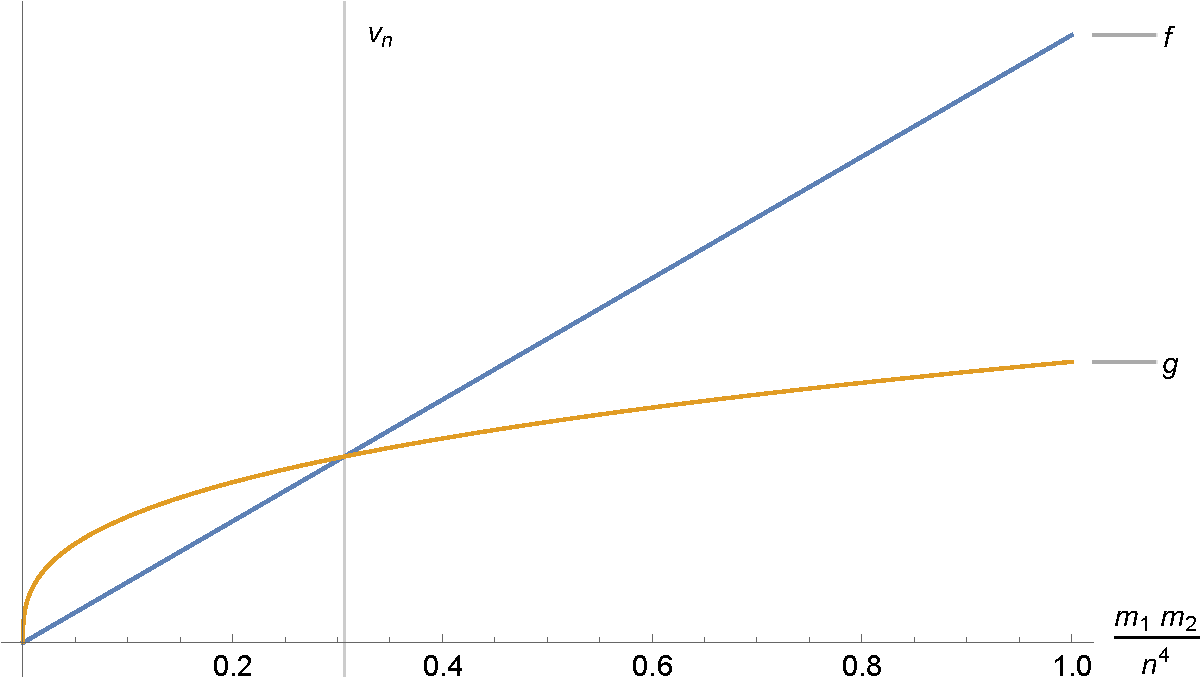
\includegraphics[width = 0.5\textwidth]{megi.pdf}
\end{center}
$$\frac{m_1m_2}{n^\alpha} = (m_1m_2)^{\frac{\beta}{\beta +1}} n ^ {\frac{2 - \alpha\beta }{\beta + 1}} \Longrightarrow  (m_1m_2)^{1-\frac{\beta}{\beta + 1}} = n^{\frac{2-\alpha\beta}{\beta + 1} + \alpha}\Longrightarrow (m_1m_2)^{\frac{1}{\beta +1}} = n^{\frac{2+\alpha}{\beta + 1}} \Longrightarrow m_1m_2 = n^{2 + \alpha} $$

This means that when $m_1m_2 \geq n^{2+\alpha}$ it is more optimal for the algorithm to have the complexity of case (d) otherwise the complexity is $\mathcal{O}(n^{v_n-\alpha}) = \mathcal{O}(n^{2+o(1)})$. \\
\end{enumerate}
Therefore considering everything since we choose the minimum $l$ then the time complexity for this algorithm is: $$\mathcal{O}\left(\min \left((m_1m_2)^{\frac{\beta}{\beta +1}} n ^ {\frac{2 - \alpha\beta }{\beta + 1}} + n^{2+o(1)}, n^{\omega+o(1)}, nm_2, nm_1 \right)\right) $$\\\
\textbf{Case: }$\mathbf{m_1 = m_2 = m}$\\\\
$$
\beta = \frac{w - 2}{1 - \alpha} \approx 0.533 \quad \alpha \approx 0.294 \quad \omega \approx 2.376
$$
$$
\frac{2\beta}{\beta + 1} \approx 0.695 \approx 0.7 \quad \frac{2-\alpha\beta} {\beta + 1} \approx 1.202 \approx 1.2
$$
Hence the complexity of this algorithm for this case is $\mathcal{O}(m^{0.7}n^{1.2} + n^{2+o(1)})$.

\break
\section*{Appendix (A) - Questions}
\subsection*{Exercise 2.1}
In the United States, coins are minted with denominations $1, 5, 10, 25,$ and $50$ cents. Now consider a country whose coins are minted with denominations of $\{d_1, d_2, \cdots, d_k\}$ units. We seek an algorithm to make change of n units using the minimum number of coins for this country.\\
\begin{enumerate}
\item (1 point) The greedy algorithm for making change repeatedly uses the biggest coin smaller than the amount to be changed until it is zero. Provide a greedy algorithm for making change of n units using US denominations. Prove its correctness and analyze its time complexity.\\
\item (1 point) Show that the greedy algorithm does not always use the minimum number of coins in a country whose denominations are $\{1, 6, 10\}$.\\
\item (3 points) Give an O(nk)-time algorithm that correctly determines the smallest number of coins needed to make change of n units using denominations {d1, d2, ..., dk} . Analyze its running time.
\end{enumerate}
\subsection*{Exercise 2.2}
We have seen Strassen's algorithm for multiplying two $n\times n$ matrices in $\mathcal{O}(n^2.81)$ time. Often in practice, the matrices to multiply are sparse, that is the number of non-zero elements in them is small. Intuitively, in this case we should be able to multiply the matrices faster. Unfortunately, Strassen's algorithm cannot use this property directly, and your task is to find a way around this.

\textbf{Notation}: Let $A,B$ be two matrices of size $n\times n$. Let $A_{*k}$ be the $k$-th column of $A$, and $A_{k*}$ be the k-th row of A for all $1 \leq k \leq n$, similarly for B. Denote the number of non-zero elements in $A_{*k}$ and $B_{k*}$ by $a_k$ and $b_k$, respectively.
\begin{enumerate}
\item (1 point) Show that $A\cdot B$ can be computed naively using $\sum ^n_{k=1}a_kb_k$ multiplications.\\
\item (1 point) Show that the number of arithmetic operations performed by the naive algorithm is $\mathcal {O}(nm)$ if $\sum ^n_{k=1}a_k\leq m$ and $\sum ^n_{k=1}b_k \leq m$.
\\
Note that computing $A \cdot B$ can be reduced to computing the product of two smaller rectangular matrices. We will use the fast rectangular matrix multiplication to speed up the calculation when the naive algorithm must perform many operations.

\textbf{Notation}: Let $M(a,b,c)$ be the smallest number of multiplications required for computing the product of two rectangular matrices of sizes $a\times b$ and $b\times c$ and $w(r,s,t)=k$ be the smallest number such that $M(n^r,n^s,n^t)=\mathcal{O}(n^{k+o(1)})$. 

The Coppersmith-Winograd bounds for $w(1,r,1)$ with $0\leq r \leq1$ are as follows:

$$w=w(1,1,1)\leq 2.376$$

$$\max \{0 \leq r\leq 1|w(1,r,1)=2\}=\alpha >0.294$$

\item (1 point) Show that $M(ap,bp,cp) \leq M(a,b,c)M(p,p,p)$ for all $a,b,c,p\in \mathcal{N}$\\

\item (2 points) Hence show that $w(1,r,1)\leq 2$ if $0\leq r\leq \alpha$, and $w(1,r,1) \leq 2+ \beta (r - \alpha)$, otherwise, where $\beta=(w-2)/(1-\alpha)$.\\

\item (2 points) Let $\pi$ be a permutation such that $a\pi (1)b_{\pi (1)} \geq a_{\pi(2)} b_{\pi(2)} \geq … \geq a_{\pi(n)}b\pi(n)$. Show that for all $1\leq l\leq n$,

$$\sum ^n_{k=l+1}a_{\pi(k)}b_{\pi(k)} \leq \frac{m_1m_2}{l}$$

where $m_1=\sum ^n_{k=1}a_k and m_2=\sum ^n_{k=1}b_k.$\\

\item (3 points) Show that the following algorithm is correct and show it complexity in terms of $n,m_1,m_2$.
\end{enumerate}

$a_k$ = the number of non-zero elements in $A_{*k}$, for $1\leq k\leq n $\\

$b_k$ = the number of non-zero elements in $B_{k*}$, for $1\leq k\leq n$ \\

$\pi$ - a permutation such that $a_{\pi(1)}b_{\pi(1)}\geq a_{\pi(2)}b_{\pi(2)}\geq\cdots \geq a_{\pi(n)}b_{\pi(n)}$\\

Find $l$ that minimizes $M(n,l,n)+\sum _{k\geq l} a_{\pi(k)}b_{\pi(k)}$\\

Let $I={\pi(1),\pi(2),\cdots,\pi(l)}$ and $J={\pi(l+1),\pi(l+2),\cdots,\pi(n)}$\\

Compute $C_1=A_{*I}B_{I*}$ using the fast rectangular matrix multiplication algorithm\\

Compute $C_2=A_{*J}B_{J*}$ using the fast rectangular matrix multiplication algorithm\\

return $C_1+C_2$\\
In particular, using the bounds for $w$ and $\alpha$, show that the complexity of the algorithm is $\mathcal{O}(m^{0.7}n^{1.2}+n^{2+o(1)})$ for $m1=m2=m$


\end{document}